\documentclass[11pt]{article}

\usepackage{../algebra}

\begin{document}

\coverpage{6}

% hw problem 1 -----------------------------------------------------------------

\newpage
\section*{Homomorphisms between clocks}
    \problem{
        Find all homomorphisms from $\Z _{12}$ to $\Z _{15}$.
    }
    \proof{

    }

% hw problem 2 -----------------------------------------------------------------

\begin{exercise}{74}{13}
    \problem{
        If $G$ is a finite abelian group of order $n$ and $\varphi : G \to G$ is defined by $\varphi (a) = a^m$ for all $a \in G$, find the necessary and sufficient condition that $\varphi$ be an isomorphism of $G$ onto itself.
    }
    \proof{

    }
\end{exercise}


% hw problem 3 -----------------------------------------------------------------

\begin{exercise}{75}{26}
    \problem{
        If $G$ is a group and $a \in G$, define $\sigma _a (g) = a g a^{-1}$.
        We saw in Example 9 of this section that $\sigma _a$ is an isomorphism of $G$ onto itself, so $\sigma _a \in A(G)$, the group of all $1-1$ mappings of $G$ (as a set) onto itself.
        Define $\psi: G \to A(G)$ by $\psi (a) = \sigma _a$ for all $a \in G$.
        Prove that \\
        \indent {\bf (a)} $\psi$ is a homomorphism of $G$ into $A(G)$. \\
        \indent {\bf (b)} $\ker \psi = Z(G)$ the center of $G$.
    }
    \proof{
        \parspace {\bf (a)} We wish to show that $\psi$ is a homomorphism.
        That is, we must show that $\psi (ab) = \psi (a) \psi (b)$ for all $a,b \in G$.
        On the LHS, we have $\psi (ab) = \sigma _{ab}$ and on the RHS we have $\psi (a) \psi (b) = \sigma _a \circ \sigma _b$.
        For the LHS to equal the RHS we must have $\sigma _{ab} (g) = (\sigma _a \circ \sigma _b) (g)$ for all $g \in G$.
        Fix any $g \in G$, then $\sigma _{ab} (g) = (ab) g (ab)^{-1} = ab g b^{-1} a^{-1} = \sigma _a (b g b^{-1}) = \sigma _a (\sigma _b (g)) = (\sigma _a \circ \sigma _b) (g)$.
        Since $g$ was arbitrary in $G$, we have shown the equality between maps $\sigma _{ab} = \sigma _a \circ \sigma _b$ which means $\psi$ is a homomorphism. \parspace
        {\bf (b)} Now we want to show that $\ker \psi = Z(G)$.
        Let's write their definitions.
        We know $\ker \psi := \{ a \in G \mid \psi (a) = id \in A(G) \} \subset G$ and that $Z(G) := \{ a \in G \mid ag = ga \text{ for all } g \in G \}$.
        We will show equality by showing inclusion in both directions.
        Going to the left, pick any $a \in \ker \psi$, then $\psi (a) = id \in A(G)$.
        Also, by definition, $\psi (a) = \sigma _a$ this gives the equality of maps $\sigma _a = id$.
        Then we have $\sigma _a (g) = id(g) = g$ for all $g \in G$.
        By definition, $\sigma _a (g) = a g a^{-1}$ so we also have $a g a^{-1} = g$ for all $g \in G$.
        Left multiplying by $a$ gives $ag = ga$ for all $g$, which is exactly the condition for membership in $Z(G)$.
        Therefore, $a \in Z(G)$ and since $a$ was arbitray in $\ker \psi$ we have the inclusion $\ker \psi \subset Z(G)$. \parspace
        We now show the other inclusion $Z(G) \subset \ker \psi$.
        Fix any $b \in Z(G)$ then $bg = gb$ for every $b \in G$.
        Left multplying by $b^{-1}$ gives the equality $b g b^{-1} = g$ for all $b \in G$.
        The LHS is exactly $\sigma _b (g)$ so we have just shown that $\sigma _b (g) = g$ for every $b$.
        But then $\sigma _b$ performs the same actions as the identity map $id \in A(G)$ so we have $\sigma _b = id$.
        Further, $\sigma _b = \psi (b)$ so we also have $\psi (b) = id \in A(G)$, which is the condition for membership in $\ker \psi$.
        By arbitrariness of $b$, we have shown $Z(G) \subset \ker \psi$.
    }
\end{exercise}

% hw problem 4 -----------------------------------------------------------------

\newpage
\section*{Heisenberg to plane}
    \problem{
        Find an epimorphism the Heisenberg group $\Heisen$ onto $\R ^2$.
    }
    \proof{
        Consider the function $\varphi : \Heisen \to \R ^2$ which maps a matrix
        $A = \begin{bmatrix} 1 & x & z \\ 0 & 1 & y \\ 0 & 0 & 1 \end{bmatrix} \in \Heisen$
        to the point $(x, y) \in \R ^2$.
        For $\varphi$ to be an epimorphism, we must verify that $\varphi$ is both surjective and a homomorphism.
        For $\varphi$ to be surjective, for every point in $\R ^2$ we must have a matrix in $\Heisen$ such that $\varphi$ maps the matrix to the point.
        For the point $(a, b) \in \R ^2$, choose the matrix
        $A = \begin{bmatrix} 1 & a & 0 \\ 0 & 1 & b \\ 0 & 0 & 1 \end{bmatrix}$.
        Then $\varphi (A) = (a, b)$ as desired.
        Now let's verify that $\varphi$ is a homomorphism.
        We must check that $\varphi (A A') = \varphi (A) \varphi (A')$ for all $A, A' \in \Heisen$.
        $$
        A A' =
        \begin{bmatrix}
            1 & x & z \\
            0 & 1 & y \\
            0 & 0 & 1
        \end{bmatrix}
        \begin{bmatrix}
            1 & x' & z' \\
            0 & 1 & y' \\
            0 & 0 & 1
        \end{bmatrix}
        =
        \begin{bmatrix}
            1 & x'+x & z'+y'x+z \\
            0 & 1 & y'+y \\
            0 & 0 & 1
        \end{bmatrix}
        $$
        On the LHS, $\varphi (A A') = (x' + x, y' + x)$.
        Then on the RHS, we have $\varphi (A) \varphi (A') = (x, y) + (x', y') = (x+x', y+y') = (x'+x, y'+y)$.
        So the LHS equals the RHS and $\varphi$ is a homomorphism.
    }

% hw problem 5 -----------------------------------------------------------------

\newpage
\section*{Klein group}
    \problem{
        Show that the group $Sym (R)$ where $R$ is a rectangle that is not a square is isomorphic to the product $\Z _2 \times \Z _2$.
    }
    \proof{
        We know the elements of $\Z _2$ so we know the elements of $\Z _2 \times \Z _2$ and the group opertion it is endowed with.
        We must explore the group $Sym (R)$.
        Certainly $Sym (R) \leq D_8$ (where $S$ is a square) for every symmetry of a rectangle is also a symmetry of a square.
        Figure \ref{fig:sym} depicts the axis of symmetries of a rectangle $R$.
        Together with the identity transformation, there are four.
        Since $Sym (R) \leq D_8$ let's give the four transformations the same names that we call them in $D_8$.
        Namely, $Sym (R) := \{ e, r^2, f, fr^2 \}$.

        \begin{figure}[h]
            \centering
            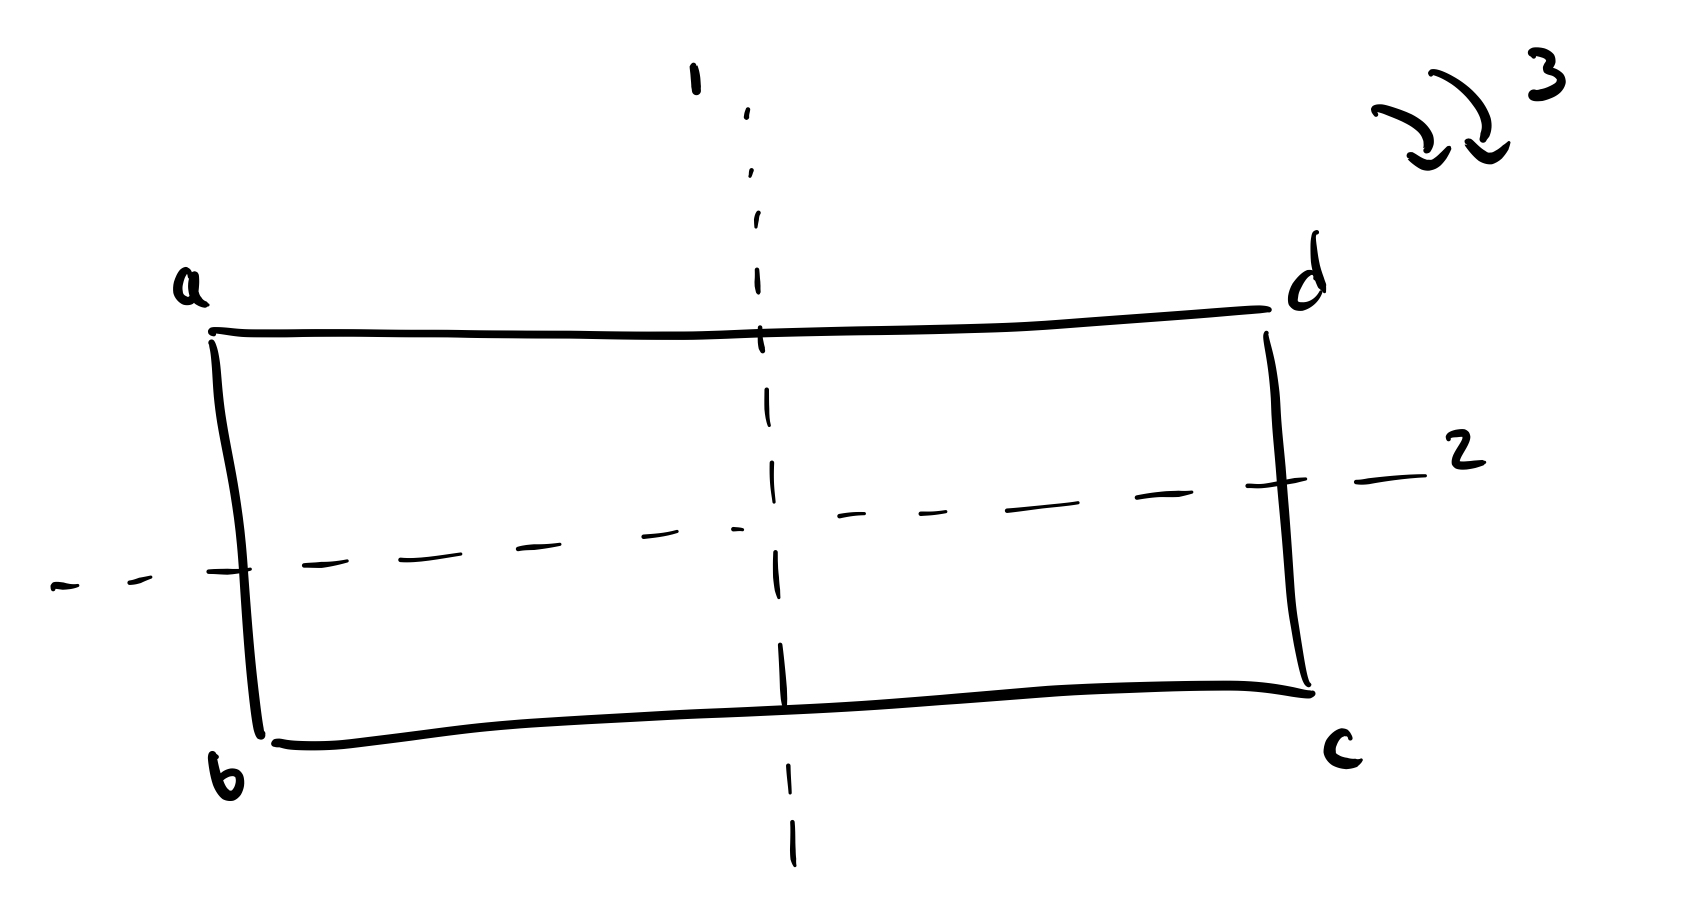
\includegraphics[width=0.5\textwidth]{img/sym}
            \caption{Symmetries of a rectangle $R$}
            \label{fig:sym}
        \end{figure}

        Figure \ref{fig:iso} defines a map $\varphi: Sym (R) \to \Z _2 \times \Z _2$.
        Just from the figure, we know that $\varphi$ is a bijection.

        \begin{figure}[h]
            \centering
            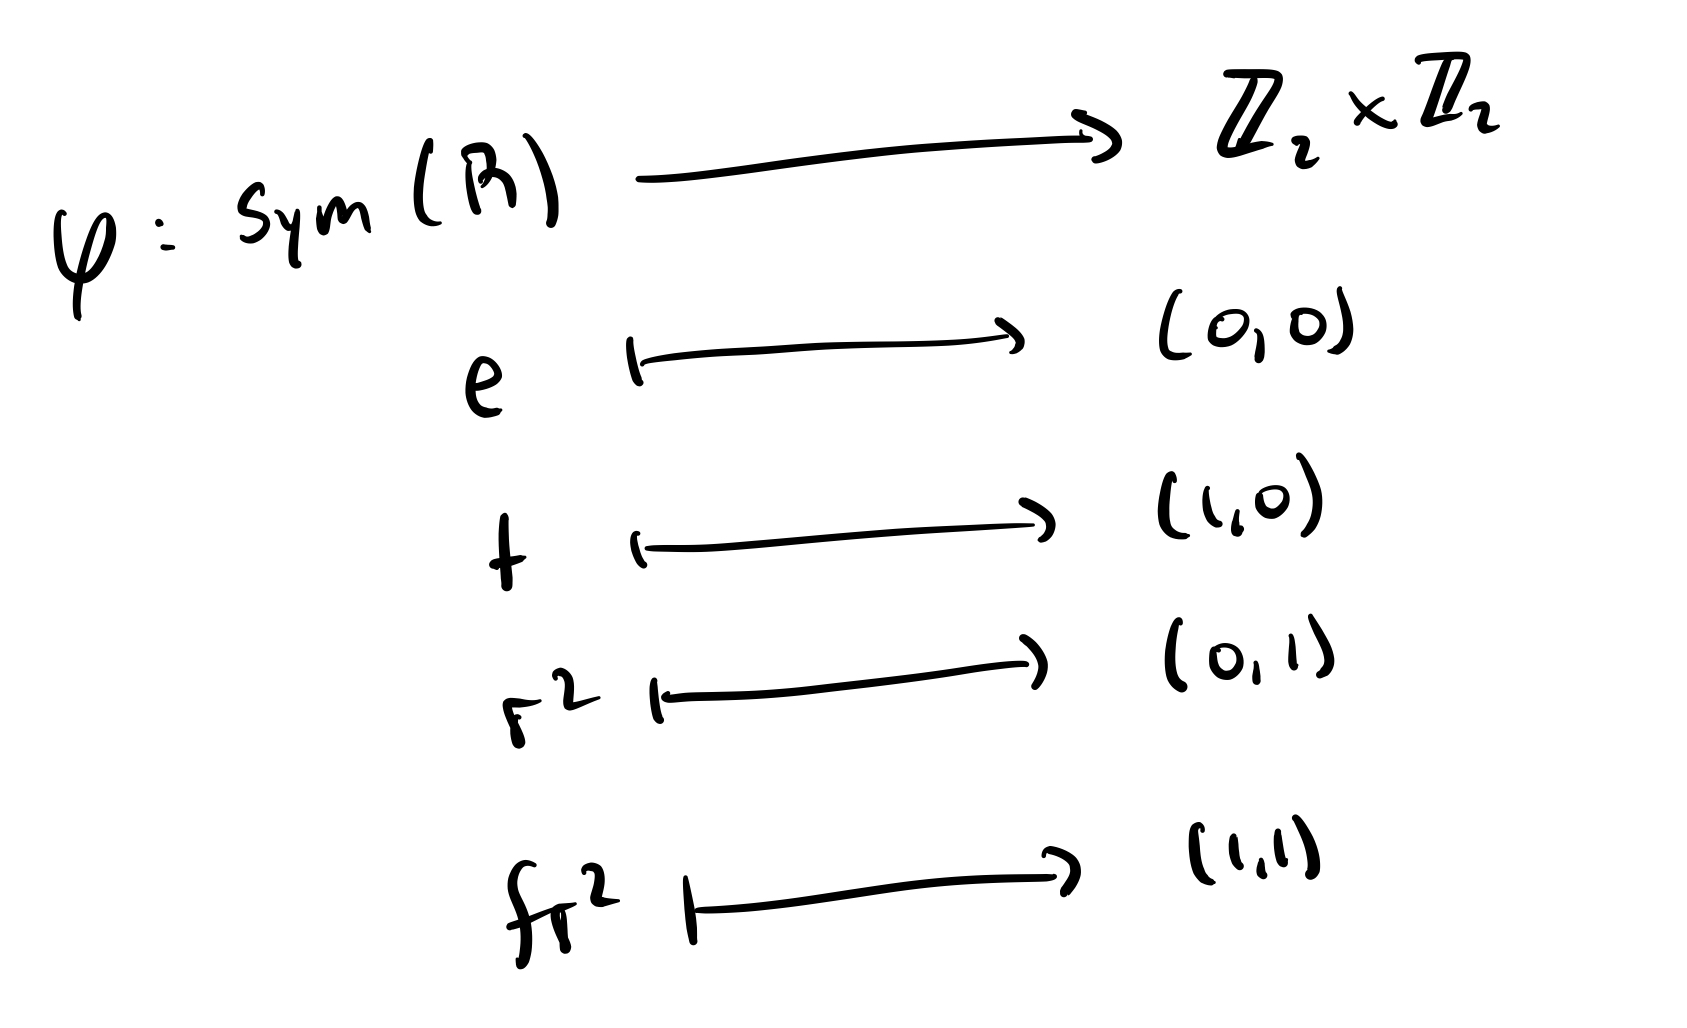
\includegraphics[width=0.4\textwidth]{img/iso}
            \caption{Isomorphism between $Sym (R)$ and $\Z _2 \times \Z _2$}
            \label{fig:iso}
        \end{figure}

        To verify that $\varphi$ is an isomorphism, we must verify that $\varphi$ is a homomorphism.
        Before doing this, note that $\Z _2 \times \Z _2$ and $Sym (R)$ are abelian.
        We can check $Sym (R)$ by verifying that $ f r^2 = r^2 f$.
        Since each group is abelian, we only need to check one ``ordering'' of each pair of elements.
        Now we verify that $\varphi$ respects the group structure.
        \begin{align*}
            \varphi (e) + \varphi (x) &= (0, 0) + \varphi (x) = \varphi (x) = \varphi (e x) \text{ for any } x \in Sym(R) \\
            \varphi (f) + \varphi (r^2) &= (1,0) + (0,1) = (1,1) = \varphi (f r^2) \\
            \varphi (f) + \varphi (fr^2) &= (1,0) + (1,1) = (0,1) = \varphi (r^2) = \varphi (ff r^2) \\
            \varphi (f r^2) + \varphi (r^2) &= (1,1) + (0,1) = (1,0) = \varphi (f) = \varphi (f r^4) \\
        \end{align*}
    }

\end{document}
